%\VignetteIndexEntry{Testing and visualizing gene overlaps with the "GeneOverlap" package}
%\VignettePackage{GeneOverlap}

\documentclass{article}

\RequirePackage{/Library/Frameworks/R.framework/Versions/3.0/Resources/library/BiocStyle/sty/Bioconductor}
\title{GeneOverlap: An R package to test and visualize gene overlaps}

\author{Li Shen\\
Contact: \email{li.shen@mssm.edu} or \email{shenli.sam@gmail.com}\\
Icahn School of Medicine at Mount Sinai\\
New York, New York}

\usepackage{Sweave}
\begin{document}
\Sconcordance{concordance:GeneOverlap.tex:GeneOverlap.Rnw:%
1 4 1 1 4 8 1 1 0 8 1 1 2 4 0 1 2 2 1 1 2 4 0 2 2 7 0 1 1 6 0 1 1 6 0 1 2 3 1 1 %
4 3 0 1 1 10 0 2 2 1 0 1 1 10 0 2 2 19 0 1 2 1 4 3 0 2 1 18 0 1 2 2 1 1 2 6 0 1 %
1 5 0 1 1 7 0 1 1 6 0 2 2 1 0 2 1 10 0 2 2 1 0 1 1 10 0 2 2 1 0 1 5 11 0 1 2 2 1 %
1 3 2 0 1 1 4 0 1 2 4 1 1 2 11 0 2 2 11 0 2 2 1 0 1 1 21 0 2 2 1 0 1 1 10 0 2 2 %
11 0 1 2 1 1 1 3 2 0 1 1 4 0 1 2 4 1 1 2 5 0 1 2 9 1 1 2 22 0 1 2 10 1}


\maketitle

\tableofcontents

\section{Data preparation} \label{sec:prep}
The \Rpackage{GeneOverlap} package is composed of two classes: \Rclass{GeneOverlap} and \Rclass{GeneOverlapMatrix}. The \Rclass{GeneOverlap} class serves as building blocks to the \Rclass{GeneOverlapMatrix} class. First, let's load the package
\begin{Schunk}
\begin{Sinput}
> library(GeneOverlap)
\end{Sinput}
\end{Schunk}
To use the \Rclass{GeneOverlap} class, create two character vectors that represent gene names. An easy way to do this is to use \Rcode{read.table("filename.txt")} to read them from text files. 

As a convenience, a couple of gene lists have been compiled into the \Robject{GeneOverlap} data. Use
\begin{Schunk}
\begin{Sinput}
> data(GeneOverlap)
\end{Sinput}
\end{Schunk}
to load them. Now, let's see what are contained in the data: there are three objects. The \Robject{hESC.ChIPSeq.list} and \Robject{hESC.RNASeq.list} objects contain gene lists from ChIP-seq and RNA-seq experiments. The \Robject{gs.RNASeq} variable contains the number of genes in the genomic background. Refer to Section~\ref{sec:data} for details about how they were created. Let's see how many genes are there in the gene lists.
\begin{Schunk}
\begin{Sinput}
> sapply(hESC.ChIPSeq.list, length)
\end{Sinput}
\begin{Soutput}
 H3K4me3  H3K9me3 H3K27me3 H3K36me3 
   13302      293     3815     4485 
\end{Soutput}
\begin{Sinput}
> sapply(hESC.RNASeq.list, length)
\end{Sinput}
\begin{Soutput}
  Exp High Exp Medium    Exp Low 
      6444       5951       7647 
\end{Soutput}
\begin{Sinput}
> gs.RNASeq
\end{Sinput}
\begin{Soutput}
[1] 20042
\end{Soutput}
\end{Schunk}
In \Rpackage{GeneOverlap}, we refer to a collection of gene lists as a gene set that is represented as a named list. Here we can see that the ChIP-seq gene set contains four gene lists of different histone marks: H3K4me3, H3K9me3, H3K27me3 and H3K36me3; the RNA-seq gene set contains three gene lists of different expression levels: High, Medium and Low. Two histone marks are associated with gene activation: H3K4me3 and H3K36me3 while the other two are associated with gene repression: H3K9me3 and H3K27me3.

\section{Testing overlap between two gene lists} \label{sec:test}
We want to explore whether the activation mark - H3K4me3 is associated with genes that are highly expressed. First, let's construct a {\tt GeneOverlap} object
\begin{Schunk}
\begin{Sinput}
> go.obj <- newGeneOverlap(hESC.ChIPSeq.list$H3K4me3, 
+                          hESC.RNASeq.list$"Exp High", 
+                          genome.size=gs.RNASeq)
> go.obj
\end{Sinput}
\begin{Soutput}
GeneOverlap object:
listA size=13302
listB size=6444
Intersection size=5833
Overlap testing has not been performed yet.
\end{Soutput}
\end{Schunk}
As we can see, the \Rclass{GeneOverlap} constructor has already done some basic statistics for us, such as the number of intersections. To test the statistical significance of association, we do
\begin{Schunk}
\begin{Sinput}
> go.obj <- testGeneOverlap(go.obj)
> go.obj
\end{Sinput}
\begin{Soutput}
GeneOverlap object:
listA size=13302
listB size=6444
Intersection size=5833
Overlapping p-value=0e+00
\end{Soutput}
\end{Schunk}
The P-value is zero, which means the overlap is highly significant. To show some more details, use the \Rfunction{print} function
\begin{Schunk}
\begin{Sinput}
> print(go.obj)
\end{Sinput}
\begin{Soutput}
Detailed information about this GeneOverlap object:
listA size=13302, e.g. DPM1 SCYL3 C1orf112 FGR FUCA2 GCLC
listB size=6444, e.g. ISG15 NOC2L KLHL17 AGRN B3GALT6 SDF4
Intersection size=5833, e.g. DPM1 C1orf112 FUCA2 SEMA3F ANKIB1 KRIT1
Union size=13913, e.g. DPM1 SCYL3 C1orf112 FGR FUCA2 GCLC
Genome size=20042
# Contingency Table:
     notA  inA
notB 6129 7469
inB   611 5833
Overlapping p-value=0e+00
Odds ratio=7.8
Overlap tested using Fisher's exact test (alternative=greater)
\end{Soutput}
\end{Schunk}
Further, we want to see if H3K4me3 is associated with genes that are lowly expressed. We do
\begin{Schunk}
\begin{Sinput}
> go.obj <- newGeneOverlap(hESC.ChIPSeq.list$H3K4me3, 
+                          hESC.RNASeq.list$"Exp Low", 
+                          genome.size=gs.RNASeq)
> go.obj <- testGeneOverlap(go.obj)
> print(go.obj)
\end{Sinput}
\begin{Soutput}
Detailed information about this GeneOverlap object:
listA size=13302, e.g. DPM1 SCYL3 C1orf112 FGR FUCA2 GCLC
listB size=7647, e.g. OR4F5 FAM138A OR4F29 PLEKHN1 C1orf170 RNF223
Intersection size=2531, e.g. FGR CFTR HS3ST1 WNT16 CYP26B1 CD38
Union size=18418, e.g. DPM1 SCYL3 C1orf112 FGR FUCA2 GCLC
Genome size=20042
# Contingency Table:
     notA   inA
notB 1624 10771
inB  5116  2531
Overlapping p-value=1
Odds ratio=0.1
Overlap tested using Fisher's exact test (alternative=greater)
\end{Soutput}
\end{Schunk}
In contrast to the highly expressed genes, the P-value is now 1 with odds ratio 0.1. 

Once a \Robject{GeneOverlap} object is created, several accessors can be used to extract its slots. For example
\begin{Schunk}
\begin{Sinput}
> head(getIntersection(go.obj))
\end{Sinput}
\begin{Soutput}
[1] "FGR"     "CFTR"    "HS3ST1"  "WNT16"   "CYP26B1" "CD38"   
\end{Soutput}
\begin{Sinput}
> getOddsRatio(go.obj)
\end{Sinput}
\begin{Soutput}
[1] 0.07461166
\end{Soutput}
\begin{Sinput}
> getContbl(go.obj)
\end{Sinput}
\begin{Soutput}
     notA   inA
notB 1624 10771
inB  5116  2531
\end{Soutput}
\begin{Sinput}
> getGenomeSize(go.obj)
\end{Sinput}
\begin{Soutput}
[1] 20042
\end{Soutput}
\end{Schunk}
It is also possible to change slots "listA", "listB" and "genome.size" after object creation. For example
\begin{Schunk}
\begin{Sinput}
> setListA(go.obj) <- hESC.ChIPSeq.list$H3K27me3
> setListB(go.obj) <- hESC.RNASeq.list$"Exp Medium"
> go.obj
\end{Sinput}
\begin{Soutput}
GeneOverlap object:
listA size=3815
listB size=5951
Intersection size=1529
Overlap testing has not been performed yet.
\end{Soutput}
\end{Schunk}
After any of the above slots is changed, the object is put into untested status. So we need to re-test it
\begin{Schunk}
\begin{Sinput}
> go.obj <- testGeneOverlap(go.obj)
> go.obj
\end{Sinput}
\begin{Soutput}
GeneOverlap object:
listA size=3815
listB size=5951
Intersection size=1529
Overlapping p-value=6.6e-53
\end{Soutput}
\end{Schunk}
We can also change the genome size to see how the p-value changes with it
\begin{Schunk}
\begin{Sinput}
> v.gs <- c(12e3, 14e3, 16e3, 18e3, 20e3)
> setNames(sapply(v.gs, function(g) {
+     setGenomeSize(go.obj) <- g
+     go.obj <- testGeneOverlap(go.obj)
+     getPval(go.obj)
+ }), v.gs)
\end{Sinput}
\begin{Soutput}
       12000        14000        16000        18000        20000 
1.000000e+00 9.998297e-01 1.381083e-05 6.169626e-25 2.769996e-52 
\end{Soutput}
\end{Schunk}

\section{Visualizing all pairwise overlaps} \label{sec:vis}
When two gene sets each with one or more lists need to be compared, it would be rather inefficient to compare them manually. A matrix can be constructed, where the rows represent the lists from one set while the columns represent the lists from the other set. Each element of the matrix then is a GeneOverlap object. To visualize this overlapping information altogether, a heatmap can be used. To illustrate, we want to compare all the gene lists from ChIP-seq with that from RNA-seq
\begin{Schunk}
\begin{Sinput}
> gom.obj <- newGOM(hESC.ChIPSeq.list, hESC.RNASeq.list, 
+                   gs.RNASeq)
> drawHeatmap(gom.obj)
\end{Sinput}
\end{Schunk}
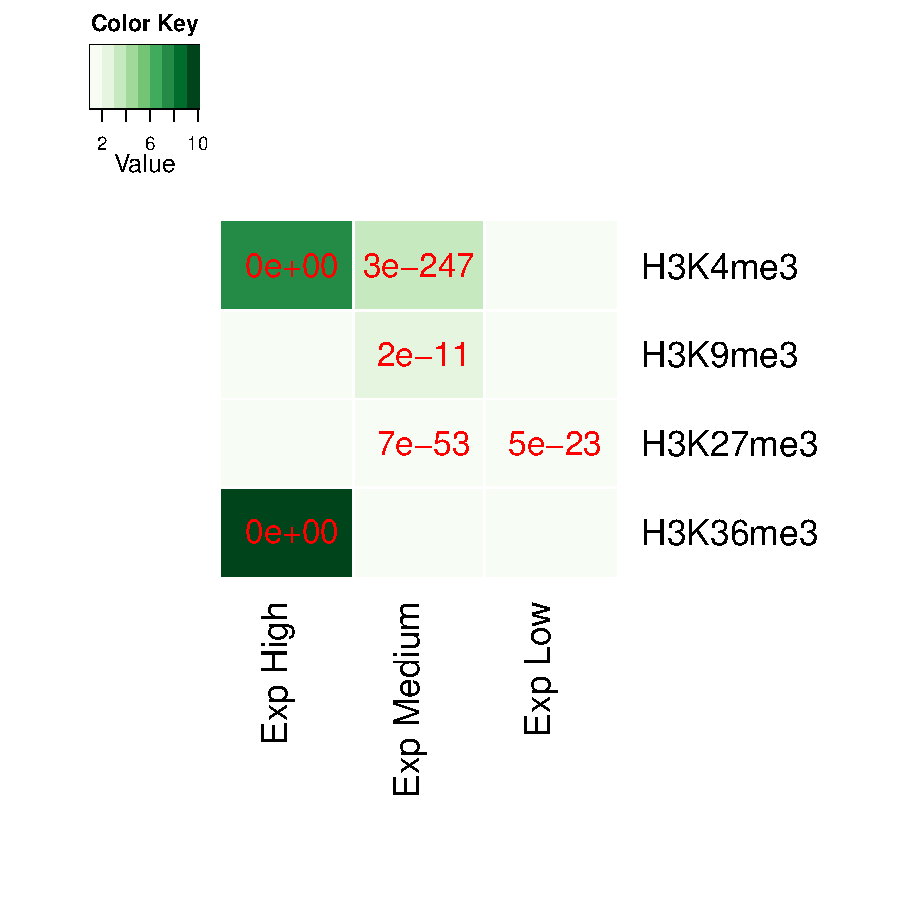
\includegraphics{GeneOverlap-013}
\begin{flushleft}
That is neat. The \Rfunction{newGOM} constructor creates a new \Rclass{GeneOverlapMatrix} object using two named lists. The colorkey represents the odds ratios and the significant p-values are superimposed on the grids.
\end{flushleft}

To retrieve information from a \Rclass{GeneOverlapMatrix} object, two important accessors are called \Rfunction{getMatrix} and \Rfunction{getNestedList}. The \Rfunction{getMatrix} accessor gets information such as p-values as a matrix, for example
\begin{Schunk}
\begin{Sinput}
> getMatrix(gom.obj, name="pval")
\end{Sinput}
\begin{Soutput}
         Exp High    Exp Medium      Exp Low
H3K4me3  0.000000 3.367287e-247 1.000000e+00
H3K9me3  0.999903  1.868791e-11 9.994000e-01
H3K27me3 1.000000  6.584807e-53 4.901011e-23
H3K36me3 0.000000  1.000000e+00 1.000000e+00
\end{Soutput}
\end{Schunk}
or the odds ratios
\begin{Schunk}
\begin{Sinput}
> getMatrix(gom.obj, "odds.ratio")
\end{Sinput}
\begin{Soutput}
           Exp High Exp Medium    Exp Low
H3K4me3   7.8338619  3.3375718 0.07461166
H3K9me3   0.6095471  2.2254522 0.66971459
H3K27me3  0.3045991  1.7855908 1.43235067
H3K36me3 10.1100840  0.7691473 0.02243317
\end{Soutput}
\end{Schunk}
The \Rfunction{getNestedList} accessor can get gene lists for each comparison as a nested list: the outer list represents the columns and the inner list represents the rows
\begin{Schunk}
\begin{Sinput}
> inter.nl <- getNestedList(gom.obj, name="intersection")
> str(inter.nl)
\end{Sinput}
\begin{Soutput}
List of 3
 $ Exp High  :List of 4
  ..$ H3K4me3 : chr [1:5833] "DPM1" "C1orf112" "FUCA2" "SEMA3F" ...
  ..$ H3K9me3 : chr [1:66] "ZNF195" "SEC63" "RNASET2" "TSSC1" ...
  ..$ H3K27me3: chr [1:563] "C1orf112" "SLC25A13" "CCDC109B" "ITGA3" ...
  ..$ H3K36me3: chr [1:3245] "DPM1" "C1orf112" "NFYA" "SEMA3F" ...
 $ Exp Medium:List of 4
  ..$ H3K4me3 : chr [1:4938] "SCYL3" "GCLC" "C1orf201" "NIPAL3" ...
  ..$ H3K9me3 : chr [1:141] "ZNF263" "ZNF200" "ERP44" "PRKCH" ...
  ..$ H3K27me3: chr [1:1529] "TMEM176A" "SLC7A2" "SARM1" "PLXND1" ...
  ..$ H3K36me3: chr [1:1147] "SCYL3" "GCLC" "CYP51A1" "ALS2" ...
 $ Exp Low   :List of 4
  ..$ H3K4me3 : chr [1:2531] "FGR" "CFTR" "HS3ST1" "WNT16" ...
  ..$ H3K9me3 : chr [1:86] "DLEC1" "ZPBP" "TRHDE" "NTN4" ...
  ..$ H3K27me3: chr [1:1723] "FGR" "HS3ST1" "WNT16" "CYP26B1" ...
  ..$ H3K36me3: chr [1:93] "CBLN4" "ZNF285" "PKD2L2" "C20orf26" ...
\end{Soutput}
\end{Schunk}
Another important accessor is the method \Rfunction{"["} that allows one to retrieve \Rclass{GeneOverlap} objects in a matrix-like fashion. For example,
\begin{Schunk}
\begin{Sinput}
> go.k4.high <- gom.obj[1, 1]
> go.k4.high
\end{Sinput}
\begin{Soutput}
GeneOverlap object:
listA size=13302
listB size=6444
Intersection size=5833
Overlapping p-value=0e+00
\end{Soutput}
\end{Schunk}
gets the \Rclass{GeneOverlap} object that represents the comparison between H3K4me3 and highly expressed genes. It is also possible to get \Rclass{GeneOverlap} objects using labels, such as
\begin{Schunk}
\begin{Sinput}
> gom.obj["H3K9me3", "Exp Medium"]
\end{Sinput}
\begin{Soutput}
GeneOverlap object:
listA size=293
listB size=5951
Intersection size=141
Overlapping p-value=1.9e-11
\end{Soutput}
\end{Schunk}

\Rclass{GeneOverlapMatrix} can also perform self-comparison on one gene set. For example, if we want to know how the ChIP-seq gene lists associate with each other, we can do
\begin{Schunk}
\begin{Sinput}
> gom.self <- newGOM(hESC.ChIPSeq.list, 
+                    genome.size=gs.RNASeq)
> drawHeatmap(gom.self)
\end{Sinput}
\end{Schunk}
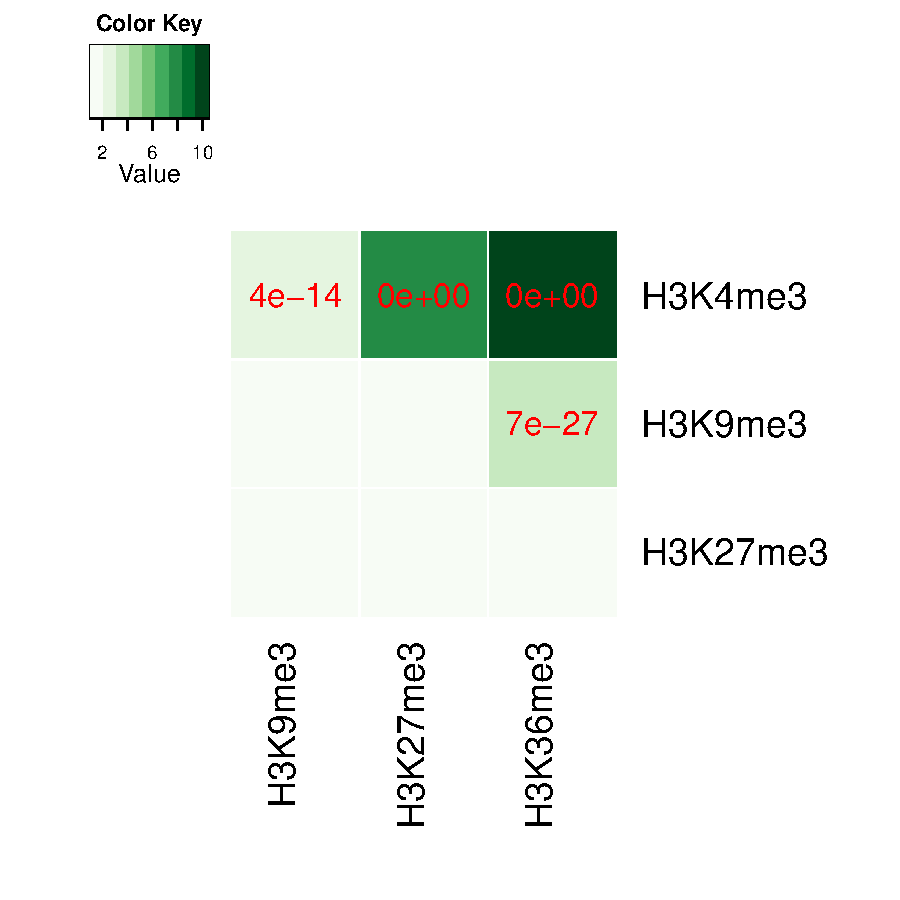
\includegraphics{GeneOverlap-019}
\begin{flushleft}
Only the upper triangular matrix is used.
\end{flushleft}

It is also possible to change the number of colors and the colors used for the heatmap. For example
\begin{Schunk}
\begin{Sinput}
> drawHeatmap(gom.self, ncolused=5, grid.col="Blues", note.col="black")
\end{Sinput}
\end{Schunk}
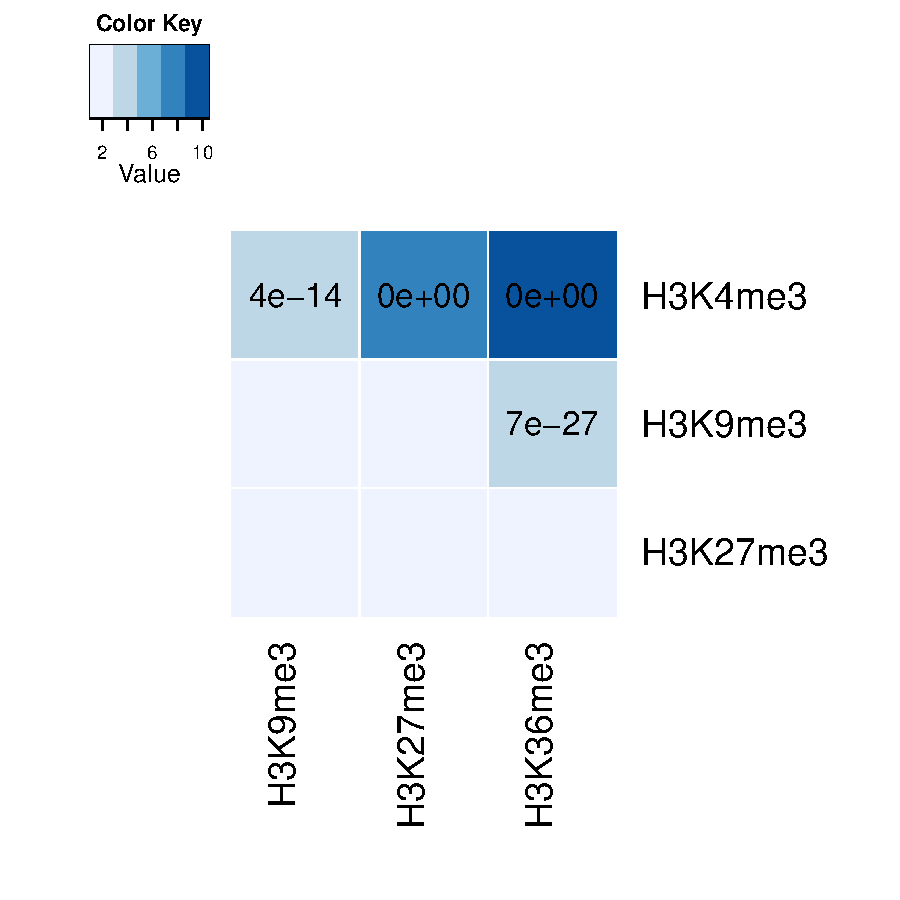
\includegraphics{GeneOverlap-020}


\section{Data source and processing} \label{sec:data}
The experimental data used here were downloaded from the ENCODE~\cite{ENCODE} project's website. Both ChIP-seq and RNA-seq samples were derived from the human embryonic stem cells (hESC). The raw read files were aligned to the reference genome using Bowtie~\cite{Bowtie} and Tophat~\cite{Tophat}. 

Cufflinks~\cite{Cufflinks} was used to estimate the gene expression levels from the RNA-seq data. The entries with duplicated gene names were removed all together to avoid ambiguity. Only protein coding genes were retained for further analysis. The genes were further filtered by FPKM status and only the genes with "OK" status were kept. This left us with 20,042 coding genes whose FPKM values were reliabled estimated. The genes were then separated into three groups: high (FPKM>10), medium (FPKM>1 and <=10) and low (FPKM<=1). 

For ChIP-seq, one replicate from IP treatment and one replicate from input control were used. Peak calling was performed using MACS2 (v2.0.10) with default parameter values. The peak lists then went through region annotation using the diffReps package~\cite{diffReps}. After that, the genes that had peaks on genebody and promoter regions were extracted. The genes were further filtered using the RNA-seq gene list obtained above.

\section{SessionInfo}
\begin{Schunk}
\begin{Sinput}
> sessionInfo()
\end{Sinput}
\begin{Soutput}
R version 3.0.1 (2013-05-16)
Platform: x86_64-apple-darwin10.8.0 (64-bit)

locale:
[1] en_US.UTF-8/en_US.UTF-8/en_US.UTF-8/C/en_US.UTF-8/en_US.UTF-8

attached base packages:
[1] stats     graphics  grDevices utils     datasets  methods   base     

other attached packages:
[1] GeneOverlap_0.2.0

loaded via a namespace (and not attached):
[1] BiocStyle_1.0.0    bitops_1.0-6       caTools_1.16       gdata_2.13.2      
[5] gplots_2.12.1      gtools_3.1.0       KernSmooth_2.23-10 RColorBrewer_1.0-5
[9] tools_3.0.1       
\end{Soutput}
\end{Schunk}

\bibliographystyle{unsrt}
\bibliography{GeneOverlap}

\end{document}






